\documentclass{article}
\usepackage{amsmath}
\usepackage{amssymb}
\usepackage{graphicx}
\usepackage[margin=1in]{geometry}
\usepackage{hyperref}
\usepackage{caption}
\usepackage{float}
\graphicspath{{images/}}
\hypersetup{
    colorlinks=true,
    urlcolor=blue,
}
\begin{document}

\title{Uncertainty of Probability}
\author{Aresh Pourkavoos}
\maketitle

Experiment with unknown probability of success $p$ \\
Prior distribution is uniform (1) over interval $[0, 1]$ \\
Conduct experiments, obtain $j$ successes and $k$ failures \\
New distribution is $p^j(1-p)^k$ (normalized to have integral 1) \\
Mean is $\frac{j+1}{j+k+2}$,
as if adding a ``virtual'' success and failure \\
May visualize all possible ``paths'' as experiments are performed
as below
\begin{center}
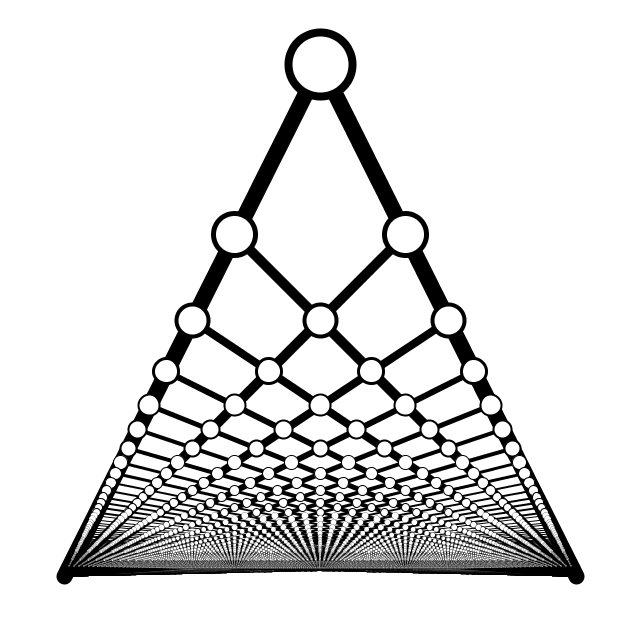
\includegraphics[width=0.5\linewidth]{grid.png}
\end{center}
Initial state is the top vertex, each experiment moves down a ``layer'' \\
Failure moves left, success moves right \\
Horizontal position is expected probability, e.g. fail-fail-succeed is
$\frac{1}{2} \rightarrow \frac{1}{3} \rightarrow \frac{1}{4} \rightarrow \frac{2}{5}$ \\
State approaches position on bottom edge corresponding to probability \\

Diagram may also be obtained by perspective transformation of a square grid \\
Straight lines are preserved: adding successes/failures moves straight \\
Start with point $(j, k, 2)$ (success, failure, unknown) \\
Normalize (make sum 1) by dividing coordinates by $j+k+2$ \\
Use coefficients to combine $(1, 0)$ (success), $(0, 0)$ (failure),
$\left(\frac{1}{2}, 1\right)$ (unknown) \\
Vertical position ranges from 0 to 1 like probability: measures ``uncertainty'' \\
Given by $\frac{2}{j+k+2}$: depends only on total number of trials \\
Horizontal position may be obtained from distribution alone:
expected value generalizes to all distributions \\
How to generalize uncertainty? \\

\end{document}
